\documentclass[a4paper]{article}
\usepackage{amsmath}
\usepackage{minted}
\usepackage{hyperref}
\usepackage[margin=2.0cm]{geometry}

\usepackage{graphicx}
\graphicspath{ {/home/ubuntu/www/octopress/source/} }
\def\title{Machine Learning: the Basics}

\begin{document}

Machine learning is the art of giving a computer data, and having it learn trends from that data and
then make predictions based on new data. While this may sound complicated, the basics turn out to be
very understandable.\\

Machine learning comes in two distinct flavors:

\begin{itemize}
    \item
        \textbf{Supervised learning:} In a supervised learning algorithm, the data is a set of training examples
        with the associated "correct answers". The algorithm learns to predict the correct answer from
        this training set. An example of this would be learning to predict whether an email is spam if
        given a million emails, each of which is labeled as "spam" or "not spam".
    \item
        \textbf{Unsupervised learning:} In an unsupervised learning algorithm, the algorithm can find trends in
        the data it is given, without looking for some specific "correct answer". Examples of
        unsupervised learning algorithms involve clustering (grouping similar data points) or anomaly
        detection (detecting unusual data points in a data set).
\end{itemize}

Supervised learning algorithms, such as neural networks and support vector machines, are what people
traditionally think of as artificial intelligence and machine learning.

Before digging in to more advanced algorithms, let's start with something simple to give you an
understanding of how many supervised learning algorithms work.

\subsection*{Your First Machine Learning Algorithm: Linear Regression}

Although it may not seem like it, linear regression - also known as least squares regression - is a
type of supervised machine learning algorithm. Suppose we have some data set $X$ and the responses, $Y$.

\[X = \begin{bmatrix}1.0 \\ 2.5 \\ 7.3 \end{bmatrix},\; Y = \begin{bmatrix}3.0 \\ 9.3 \\ 19.5 \end{bmatrix}\]

We want to develop the best linear model \(\hat{y}\) of two parameters which predicts the value of \(y\) given the value of \(x\):

\[\hat{y} = \beta_0+ \beta_1 x.\]

A common definition of "best" in this context is the model which minimizes the sum of squared residuals. (The residual of a data point is the difference between the actual value and the predicted value). Note that since the parameters \(\beta\) control the predictions, the residuals - and the sum of squared residuals - depends entirely on these two parameters. This idea of minimizing some function (in this case, the sum of squared residuals) is a building block of supervised learning algorithms, and in the field of machine learning this function - whatever it may be for the algorithm in question - is referred to as the cost function. In this case, we have the cost function J defined as follows:\[J(\beta_0, \beta_1)  = \sum_{(x_i, y_i) \in X\times Y} (y_i - \hat{y}(x_i))^2 = \sum_{(x_i, y_i) \in X\times Y} \left(y_i - (\beta_0 + \beta_1 x_i)\right)^2\]

Thus, the goal of our supervised learning algorithm is to find the \(\beta_0\) and \(\beta_1\) which minimize \(J(\beta_0, \beta_1)\). We can do that quickly and easily via an algorithm known as gradient descent, which is a generic algorithm used to minimize any function.

(\emph{Note: gradient descent can only find local minima, but luckily, the cost function for linear
regression is convex and the local and global minima are the same.})

\subsection*{Gradient Descent}

There is an incredibly simple way to minimize a multivariable function iteratively: gradient
descent. As you may remember from your calculus class, the gradient of a function $g(x, y)$ is
\[\nabla g(x, y) = \begin{bmatrix} \frac{\partial g}{\partial x} \\ \frac{\partial g}{\partial
    y}\end{bmatrix}.\]

More importantly, however, the gradient of a function is a vector which points towards the direction
of maximum increase. Consequently, in order to minimize a function, we just need to take the
gradient, look where it's pointing, and head the other direction. Thus, gradient descent can be
succinctly described in just a few steps:

\begin{itemize}
    \item
        Choose a random starting point for your variables. For performance reasons, this starting
        point should really be \emph{random} - use a pseudorandom number generator to choose it.
    \item
        Take the gradient of your cost function at your location.
    \item
        Move your location in the opposite direction from where your gradient points, by just a bit.
        Specifically, take your gradient \(\nabla g\), and subtract \(\alpha \nabla g\) from your variables,
        where \(\alpha\) is just some small number (0.1? 0.5? 0.01?) that you can tune to adjust how fast
        your algorithm runs.
    \item
        Repeat steps 2 and 3 until you're satisfied and repeating them more doesn't help you too much.
\end{itemize}

Using gradient descent with a few hundred iterations, we can easily find parameters \(\beta\) for our linear regression which give us a nice fit. (Note that there are faster algorithms than gradient descent, but they operate on the same basic principles!)

Here is a series of graphs of data points and lines of best fit that are generated by running
gradient descent for a different number of iterations. Note how with each iteration, the line fits
the data better.

\begin{center}
    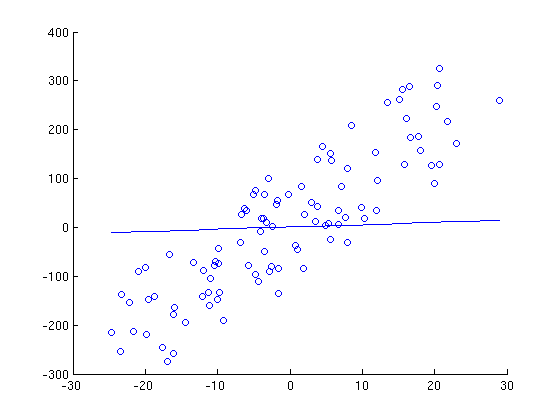
\includegraphics[scale=0.5]{images/0.png}\\
    0 Iterations (Randomly chosen parameters)
\end{center}

\begin{center}
    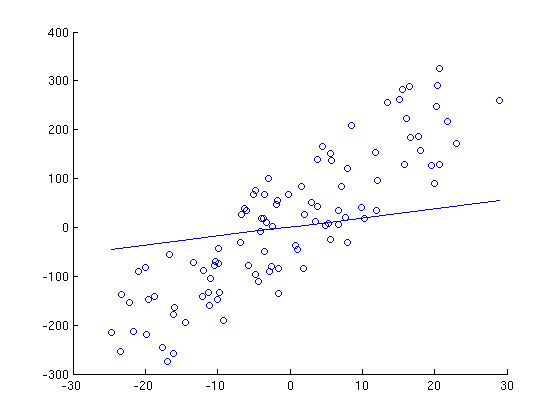
\includegraphics[scale=0.5]{images/2.png}\\
    2 Iterations
\end{center}

\begin{center}
    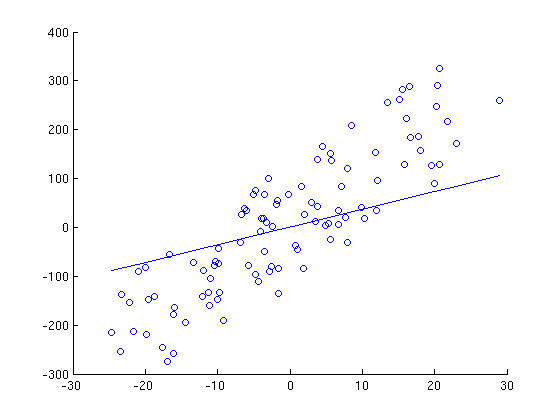
\includegraphics[scale=0.5]{images/5.png}\\
    5 Iterations
\end{center}

\begin{center}
    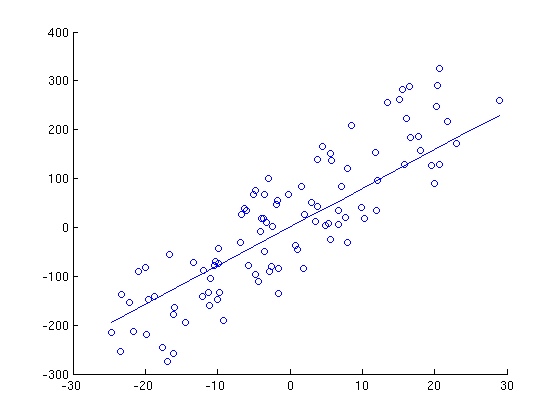
\includegraphics[scale=0.5]{images/20.png}\\
    20 Iterations
\end{center}

\begin{center}
    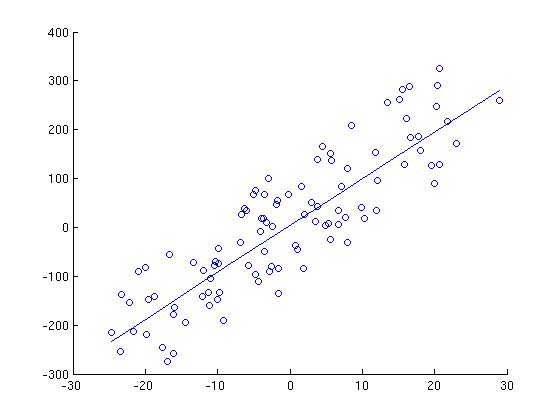
\includegraphics[scale=0.5]{images/500.png}\\
    500 Iterations
\end{center}

Those of you that are well-versed in statistics will call me out and say that this is a silly way to
find the least squares regression line, as you can set up and solve a system of equations to do it.
This is completely true, and I am using linear regression to demonstrate these basic ideas. However,
note that setting up a system of equations and solving it becomes computationally intractable once
you are doing multiple linear regression with thousands of different variables and millions of data
points, and at that scale running an iterative learning algorithm along the lines of gradient
descent will be much, much faster.

\subsection*{Final Note}

Although conceptually, linear regression via gradient descent is a simple algorithm, the basic
concepts are the same as those for much more advanced learning algorithms, such as neural networks.
These algorithms simply replace the linear model with a much more complex model - and,
correspondingly, a much more complex cost function. Eventually, I'll get around to writing about the
models and cost functions used in neural networks.
\end{document}
